\chapter{Related work} \label{chap:related_work}
In this chapter we will go in-depth discussing common approaches that are being used in the group recommendation task. We introduce the main differences between basic types  and go through simple as well as more advanced methods.\newline

We assume that we have individual user preferences (if group preferences are available, then the task actually becomes a simple recommendation with the group acting as a single user). Therefore it is necessary to make a distinction based on where the algorithm goes from preference of group's individual users to a result for the whole group.
\begin{itemize}
    \item \textbf{Aggregate models} \newline
    The aggregation works on merging preferences of each member of the group into a single set of preferences that can be then directly consumed by a recommender system, therefore creating a group preference model. Aggregating the single-user preferences either directly by aggregating ratings of seen, or and rated items, or by aggregating the extracted models of user preference to create a single model for the whole group, such as preference matrix in matrix factorization approaches, text descriptions, or item-based recommendations and so on, we will discuss these techniques later.
    
    % Aggregates the models for RS. Recommender is working on a set of already aggregated group preferences, either directly aggregating ratings of seen items, or more high level extracted features such as preference matrix in matrix factorization approaches, text description for item-based recommendations and so on, we will discuss these techniques later.
    
    This aggregation step precedes the recommendation step. We can see a visualization in figure \ref{fig:before_rec_agg}.
    
    
    \item \textbf{Aggregate predictions} \newline
     Aggregates predictions outputted from RS. Recommender recommends separately for each member of the group based solely on their single-user preferences. Then the resulting recommended items are aggregated together to a single list of recommendations for the whole group. There are two main ways how the final list can be created. Either directly take items each user likes and append them together in some specified manner, or calculate some common utility function from all recommended items and select those that are the most fitting to the group based on this utility function. We will discuss both in more detail in the section \ref{sec:03_simple_aggregation_metods}.
     
     Aggregation step follows after the actual recommendation step. We can see a visualization of this approach in figure \ref{fig:after_rec_agg}.
     
    \item \textbf{Aggregation is an uniform part of the recommender} \newline
    In this case the algorithm directly works with users of of the group and does not allow for a clear distinction of the aggregation step. It is deeply and inseparably built into the algorithm it self. Sometimes the perception of inseparability of these two steps can vary in the literature. Some could say that for example aggregating the user profiles in matrix factorization makes the aggregation inseparable, because there is a specific reprocessing done before the aggregation step. But others will point out, that the user latent matrix is just a representation of a user preference, even if processed by the algorithm it self. We will let the reader decide for them selves where they see the distinguishing border. We will briefly discuss the available methods in section \ref{sec:03_advanced_aggregation_methods}
\end{itemize}

\begin{figure}[htbp]
    \centering
    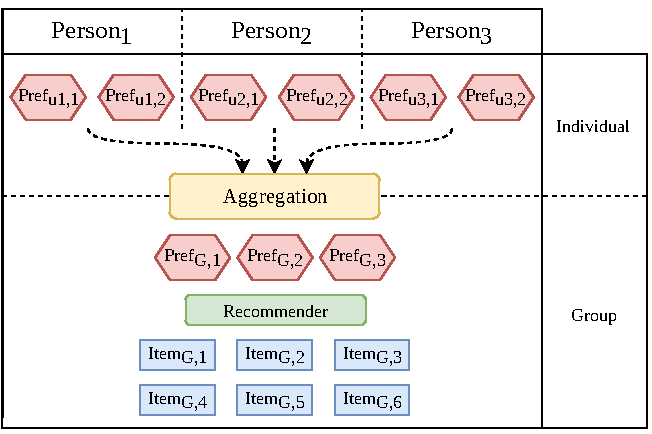
\includegraphics{img/before-rec-aggregation.pdf}
    \caption{High level overview of group recommendation with aggregation of individuals' preferences, before recommendation.}
    \label{fig:before_rec_agg}
\end{figure}

\begin{figure}[htbp]
    \centering
    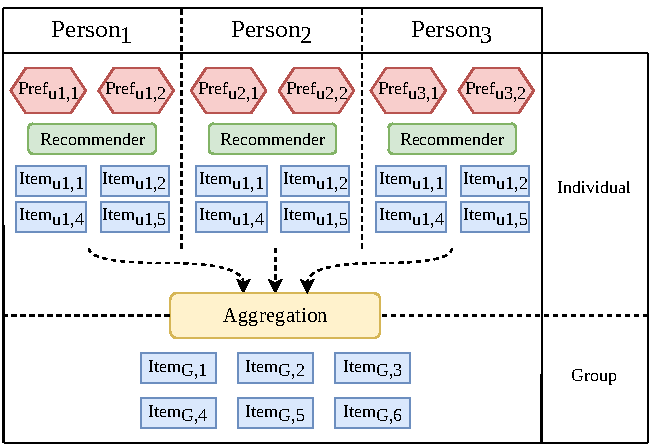
\includegraphics{img/after-rec-aggregation.pdf}
    \caption{High level overview of group recommendation with aggregation on top of recommendation results for individual users.}
    \label{fig:after_rec_agg}
\end{figure}



\section{Simple aggregation methods}\label{sec:03_simple_aggregation_metods}
We will now introduce the main aggregation functions used, together with a overview of how they interact with the single recommender systems introduced in chapter \ref{subsec:01_rec_sys.main_alg_approaches}
\subsection{Methods}
The common aggregation methods as mentioned in \cite{grouprecommendersystems_felfernig2018group}, \cite{masthoff_2011_group_rec_systems} and \cite{masthoff_2004_group_modeling} are:
\begin{itemize}
    \item \textbf{Additive utilitarian} (ADD)\newline
    Sum of score for an item across the group
    \item \textbf{Approval Voting} (APP)\newline
    Number users that like the item above certain threshold
    \item \textbf{Average} (AVG)\newline
    Average of score for an item across the group
    \item \textbf{Average without Misery} (AVM)\newline
    Average of score for an item across the group only if item is above certain threshold for all group members
    \item \textbf{Borda count} (BRC)\newline
    Sum of score derived from item raking in individual user's list
    \item \textbf{Copeland rule} (COP)\newline
    Difference between number of wins and looses for pair-wise comparison of all items
    \item \textbf{Fairness} (FAI)\newline
    
    \item \textbf{Least misery} (LMS)\newline
    \item \textbf{Majority Voting} (MAJ)\newline
    \item \textbf{Most Pleasure} (MPL)\newline
    \item \textbf{Most Respected Person} (MRP)\newline
    \item \textbf{Multiplicative} (MUL)\newline
    \item \textbf{Plurality Voting} (PLU)\newline
\end{itemize}
\subsection{Usage}

\section{Advanced aggregation methods}\label{sec:03_advanced_aggregation_methods}
\subsection{GFAR}

\section{Direct model methods}